\errorcontextlines9999
\documentclass[parskip=half]{scrartcl}

\usepackage[T1]{fontenc}
\usepackage[utf8]{inputenc}
\usepackage[english]{babel}

\usepackage[glows]{tikzpingus}
\usepackage[linkcolor=pingu@purple,urlcolor=pingu@purple,colorlinks,breaklinks,pdfusetitle]{hyperref}
\urlstyle{same}
\expandafter\def\expandafter\UrlBreaks\expandafter{\UrlBreaks\do-}

\usepackage[tex]{listings}
\usepackage[most]{tcolorbox}
\usepackage{imakeidx,tikz,fontawesome,csquotes,enumitem,microtype,tikzducks,datatool,relsize,multicol,footnotebackref}
\deffootnote{1.5em}{1em}{\textsuperscript{\hyperref[\BackrefFootnoteTag]{\thefootnotemark}}\thinspace}
\def\thefootnote{$\langle$\arabic{footnote}$\rangle$}

\newlist{inlist}{enumerate*}{1}
\setlist[inlist]{itemjoin={{,\space}},itemjoin*={{, and }},label=$\roman*$),mode=boxed}
\let\say\enquote
\def\DTLlistformatoxford{,}
\def\DTLandname{and}
\def\DTLlistformatitem#1{\textit{#1}}
\newcommand*\typesetselection[1][]{\begingroup\ifx!#1!\else\def\DTLlistformatitem##1{#1}\fi\dotypesetselection}
\def\dotypesetselection#1{\expandafter\DTLformatlist\expandafter{\csname @pingu@#1@\endcsname}\endgroup}
\usepackage{lmodern,CrimsonPro}

\addtokomafont{sectioning}{\color{gray}}
\addtokomafont{title}{\color{pingu@purple}}
\addtokomafont{author}{\normalsize}
\addtokomafont{date}{\normalsize}

\lstdefinestyle{lstpingu}{%
	tabsize=2, breaklines,
	basicstyle=\relsize{-.8}\ttfamily,
	commentstyle={\color{gray}\slshape},
	columns=fullflexible,
	emphstyle=\slshape,
	emphstyle=[2]\color{pingu@blue!80!black}\slshape,
	emphstyle=[3]\color{gray!75!white},
	emphstyle=[4]\color{pingu@blue!40!black},
	texcsstyle=*\color{gray}\bfseries,
	texcsstyle=*[2]\color{pingu@purple}\bfseries,
	lineskip=2.75pt,
	moredelim=[s][\itshape]{<}{>}
}
\lstset{style=lstpingu}
\def\ipingu#1{\lstinline'#1'}

\lstdefinelanguage{pingulang}{
	language={[LaTeX]TeX},
	moreemph={tikzpicture},
	alsoletter={.-!:2},
	moreemph=[2]{left,right,wing,eye,wings,tie,bow,none,eyes,shiny,wink,wave,grab,hug,wave,cup,straw,xshift,yshift,meta,dots,name,heart,shock,bill,hair,hairstyle,feet,foot,simple,flat,angry,back,devil,normal,princess,crown,silver,medal,patch,halo,glow,thick,2d,sunglasses,gem,shade,round},
	moreemph=[4]{:line,:ghost,parts,:devil,:back},
	moretexcs=[2]{pingu,duck,node,pingudefaults,pingudefaultsappend},
	moreemph=[3]{!hide}
}

\tcbset{%
	colframe=gray,enhanced,breakable,
	arc=2mm, arc is angular,
	fonttitle=\bfseries,
	sidebyside,
	listing options={style=lstpingu,language=pingulang},
	center lower,
	righthand width=5cm,
	bottom=0pt,top=0pt,
	before lower app={\parskip.5cm},
}
\lstMakeShortInline[style=lstpingu]{|}

\def\TikZ{Ti\textit{k}Z}
\def\tikzpingus{\TikZ pingus}

\title{The \texorpdfstring{\tikzpingus}{tikzpingus} package}
\subtitle{penguins in \TikZ}
\author{%
	\texorpdfstring{Florian Sihler\\[0.4em]
		\url{https://github.com/EagleoutIce/tikzpingus}
	}{Florian Sihler}}
\date{Version v1.0 \textendash\ 2021/07/02}

\begin{document}
\maketitle

\section{Motivation}
For my slides at university, I started to use the fairly famous \LaTeX-package \textsl{\href{https://github.com/samcarter/tikzducks}{tikzducks}} a few years ago.
Yet, it seemed somewhat of a necessity to extend the range of available \say{cute} animals in \LaTeX.
Therefore I started writing this package: \textsl{tikzpingus}.\footnote{Why \say{pingu} and not \say{pengu}? Well, this is the third try on achieving cute penguins without using any templates or vector formats as a basis. As a german, the short form \say{pingu} was merely a typo that originated from the german word \say{pinguin} for \say{penguin}. It somewhat sticked\ldots}

\textit{Please note: } While tikzpingus is certainly inspired by tikzducks, it does offer a different set of features (e.g. multiple arm positions,~\ldots).

I would be happy for any feedback or issues on the \href{https://github.com/EagleoutIce/tikzpingus}{tikzpingus}-GitHub.

\subsection{Dependencies}

As this package is constantly work in progress, the concrete dependencies may change any time.
At the moment, it only loads \TikZ, which loads a lot of other packages (e.g. |xcolor|).
Furthermore, the following \TikZ-Libraries are in use:\footnote{A lot of the libraries loaded are important only for specific extras. I plan on cleaning them up.}
\begin{inlist}
	\item |intersections|
	\item |shadings|
	\item |patterns.meta|
	\item |decorations.pathmorphing|
	\item |shapes.symbols|
\end{inlist}.

\subsection{Copyright}

Copyright \textcopyright\ \texttt{Florian Sihler}. Permission is granted to copy, distribute and\slash or modify this software under the terms of the LaTeX project public licence, version 1.3c or later \url{http://www.latex-project.org/lppl.txt}.

The shown example penguins are purely fictional characters, any resemblance to real penguins or persons is purely coincidental and no copyright infringement is intended.

\section{Usage}

If you just want a penguin, use the following syntax:
\begin{tcblisting}{title={One small penguin}}
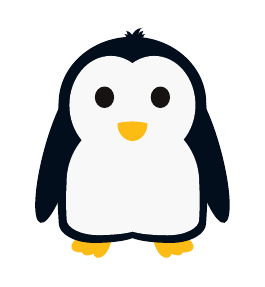
\begin{tikzpicture}
	\pingu
\end{tikzpicture}
\end{tcblisting}

There are \textit{a lot} of configuration-options which can be passed as an optional argument via the known |<key>=<value>|-style.
% TODO: click reference to full list; TODO: glow option
\begin{tcblisting}{title={Happy penguin with cup!}}
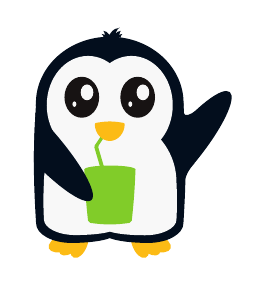
\begin{tikzpicture}
	\pingu[left wing wave, right wing grab,
	       eyes shiny, cup]
\end{tikzpicture}
\end{tcblisting}
Please note, that \say{left} and \say{right} have been chosen from the penguin-perspective.

Besides the keys defined by this package, you can use the keys of \TikZ\ and |pgf| as well (the duck was generated by the lovely \href{https://github.com/samcarter/tikzducks}{tikzducks} package):
\begin{tcblisting}{title={The Reunion}}
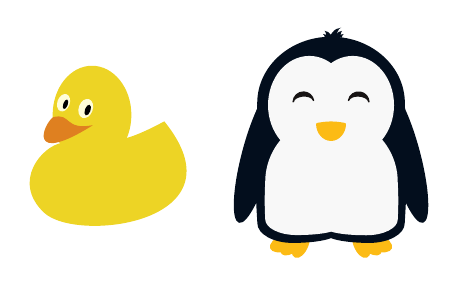
\begin{tikzpicture}
	\duck
	\pingu[xshift=3cm, yshift=14mm,
	       eyes wink]
\end{tikzpicture}
\end{tcblisting}
\subsection{Using the Coordinates}
While there are a lot of gadgets available already,
every penguin is accompanied by \textit{a lot} of adaptive coordinates
to place custom items, texts,~\ldots\ % TODO: links
They can be placed by the meta-dots option and change their positions, angles,~\ldots\ depending on other options.
Furthermore, some extras create further coordinates themselves!
All coordinates are available with |<pigu-name>-<coordinate>|.
While the default name of a penguin is \say{pingu}, it can be
changed with the name option:
\begin{tcblisting}{title={Lotta dots}}
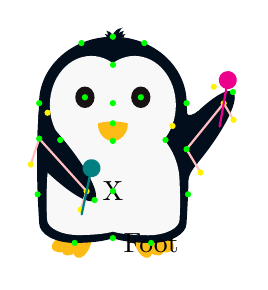
\begin{tikzpicture}
	\pingu[meta dots,left wing wave,
	       right wing grab, name=paula]
	\node at (paula-belly-center) {X};
	\node at (paula-foot-left) {Foot};
\end{tikzpicture}
\end{tcblisting}
Lets look at those coordinates in more detail (all labels are to be prefixed by |<pingu-name>-|):
\newsavebox\pinguwingright
\savebox\pinguwingright{%
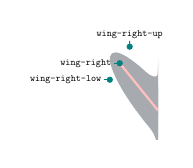
\begin{tikzpicture}%
	\scope
	\path[clip] (0,-.7) rectangle (-1,.7);
	\pgfonlayer{foreground}\path[clip] (0,-.7) rectangle (-1,.7);\endpgfonlayer
	\pingu[@block/.append style={fill=#1!35!white}, wings wave,eyes shiny,heart=gray!30!white,feet=none]
	\path[draw,pink,thick] (pingu-wing-right-start) -- (pingu-wing-right);
	\endscope
	\foreach \c/\a in {wing-right/left,wing-right-low/left,wing-right-up/above} {
		\path[fill=teal] (pingu-\c) circle [radius=1.125pt];
		\node[\a=.75mm,font=\ttfamily,scale=.35,inner sep=2.5pt] (expl-\c) at (pingu-\c) {\c};
		\draw[teal,thin] (expl-\c) -- (pingu-\c);
	}
\end{tikzpicture}%
}
\makeatletter
\newsavebox\pinguwingleft
\savebox\pinguwingleft{%
\begin{tikzpicture}%
	\scope
	\path[clip] (\pingu@w@half*2,-.7) rectangle ++(1,1.4);
	\pgfonlayer{foreground}\path[clip] (\pingu@w@half*2,-.7) rectangle ++(1,1.4);\endpgfonlayer
	\pingu[@block/.append style={fill=#1!35!white}, wings wave,eyes shiny,heart=gray!30!white,feet=none]
	\path[draw,pink,thick] (pingu-wing-left-start) -- (pingu-wing-left);
	\endscope
	\foreach \c/\a in {wing-left/left,wing-left-low/below,wing-left-up/above} {
		\path[fill=teal] (pingu-\c) circle [radius=1.125pt];
		\node[\a=.75mm,font=\ttfamily,scale=.35,inner sep=1.5pt] (expl-\c) at (pingu-\c) {\c};
		\draw[teal,thin] (expl-\c) -- (pingu-\c);
	}
\end{tikzpicture}%
}

\begin{center}
	\resizebox{.9\linewidth}!{
		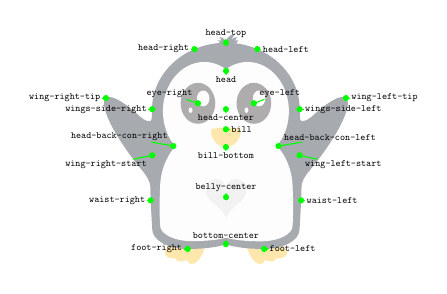
\begin{tikzpicture}
			\pingu[@block/.append style={fill=#1!35!white}, wings wave,eyes shiny,heart=gray!30!white]
			\pgfonlayer{foreground}
			\foreach \c/\a in {belly-center/above,head/below,head-top/above,foot-left/right,foot-right/left,eye-right/above left,eye-left/above right,bill/right,bill-bottom/below,wings-side-left/right,wings-side-right/left,wing-left-start/below right,wing-left-tip/right,wing-right-start/below left,wing-right-tip/left,head-right/left,head-left/right,head-center/below,head-back-con-left/above right,head-back-con-right/above left,bottom-center/above,waist-left/right,waist-right/left} {
				\path[fill=green] (pingu-\c) circle [radius=1.125pt];
				\node[\a=.5mm,font=\ttfamily,scale=.35,inner sep=1.5pt] (expl-\c) at (pingu-\c) {\c};
				\draw[green,thin] (expl-\c) -- (pingu-\c);
			}
			\endpgfonlayer
		\end{tikzpicture}
	}
\end{center}

\paragraph{The Wings}
This view excluded a lot of special data collected on the wings!
While there is more information stored for each wing, the following three coordinates are the most important to place items into penguins hand:
\begin{center}
	\null\hfill\parbox[c]{2.5\wd\pinguwingright}{\scalebox{2.5}{\usebox\pinguwingright}}\hfill\parbox[c]{4cm}{\centering\scriptsize\color{gray}\sffamily And yes, the wings are deliberately placed asymmetrical.\endgraf}\hfill
	\parbox[c]{2.5\wd\pinguwingleft}{\scalebox{2.5}{\usebox\pinguwingleft}}\hfill\null
\end{center}

\subsection{Colors}
A lot of options allow for a color to passed. In general, you can provide any color that \TikZ\ is happy with! Yet, there are some predefined pingu-colors shipped with this package, and there is one special \say{color}:
\begin{multicols}{4}
\begin{itemize}
	\foreach \col in {main,black,silver,bronze,white,yellow,lightblue,blue,green,red,purple} {
		\item[{\tikz[baseline=-.6ex]{\fill[pingu@\col,semithick,draw=black] circle (4pt);}}] \small\texttt{pingu@\col}
	}
	\item[] % buffer
\end{itemize}
\end{multicols}
Furthermore, there is the color {\makeatletter\say{\expandafter\ipingu\expandafter{\@pingu@none}}} which is available for most\footnote{Why just \say{most}? Well, this package is work in progress and I have added the option late, so I may have forgotten to patch some keys.} extras and wing-items. This color prohibits the compartments from being drawn. To be more precise, the package defines the macro |\pingu@none|, which is matched against the selected color.

As an example, lets take a look at the \say{cup}-extra, which provides an additional key \say{cup straw} to color the straw:
\begin{tcblisting}{title={Cup without a straw}}
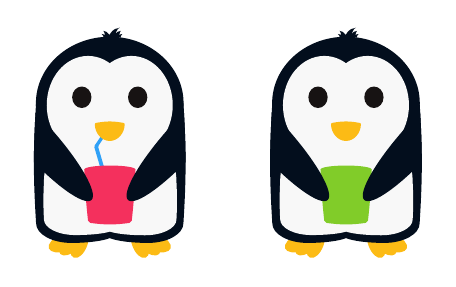
\begin{tikzpicture}
	\pingu[wings grab, cup=pingu@purple,
	       cup straw=pingu@blue]
	\pingu[wings grab, cup, xshift=3cm,
	       cup straw=!hide]
\end{tikzpicture}
\end{tcblisting}

\subsection{Setting the defaults}
You do not have to state every key for every penguin.
With the two macros \lstinline[language=pingulang]'\pingudefaults' and \lstinline[language=pingulang]'\pingudefaultsappend' (works the same, but will extend the current options) you can set default-options for all penguins to come:
\begin{tcblisting}{title={Change the mainstream}}
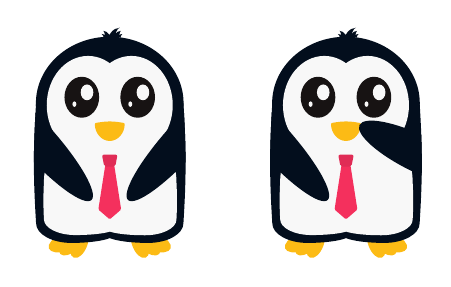
\begin{tikzpicture}
	\pingudefaults{wings grab, eyes shiny,
	  tie=pingu@purple}
	\pingu
	\pingu[left wing shock, xshift=3cm]
\end{tikzpicture}
\end{tcblisting}

\subsection{Changing the wings}
As already demonstrated, it is possible to change the wing positions!
All selected wing-items will adapt to the wing-position (although not all wing-items will make sense with every wing-position).
Currently, there are the following wing-positions:
\typesetselection{leftwing}. \say{none} is a special wing-position: it omits the drawing of wings (teaser: every selection has a none-option, which prohibits the part from being drawn)!

For each valid wing-position you can use |wings <position>| to change both wings or |left wing <position>| and |right wing <position>| to change only one wing respectively. The default wing-position is \say{normal}. If you supply more than one option for a wing, only the last one will survive.\footnote{For the sake of completeness: \ipingu{wings <position>}, \ipingu{left wing <position>}, and \ipingu{right wing <position>} are just alternatives that i prefer over the underlying mechanism: \ipingu{wings=<position>}, \ipingu{left wing=<position>} and \ipingu{right wing=<position>}.}
\begin{tcblisting}{sidebyside=false, title=Wing-Showcase}
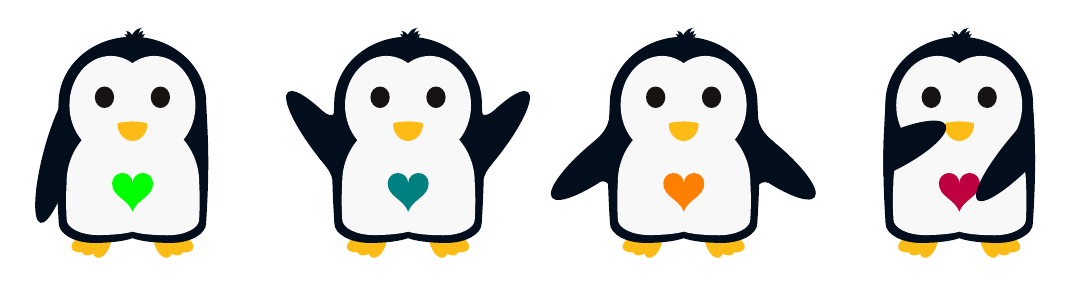
\begin{tikzpicture}
	\pingu[left wing none, heart=green]
	\pingu[wings wave, heart=teal,    xshift=3.5cm]
	\pingu[wings hug,  heart=orange,  xshift=7cm]
	\pingu[left wing grab, right wing shock, heart=purple,  xshift=10.5cm]
\end{tikzpicture}
\end{tcblisting}

\subsection{Changing the eyes}
Just like the wings, there are a couple of different eye-styles to choose from: \typesetselection{lefteye}. Just like the wings, there is a \say{none} and a \say{normal}-option (which is the default).
Furthermore, the convenient selectors |eyes <style>|, |left eye <style>|, and |right eye <style>| exist as well:
\begin{tcblisting}{sidebyside=false, title=Eye-Showcase}
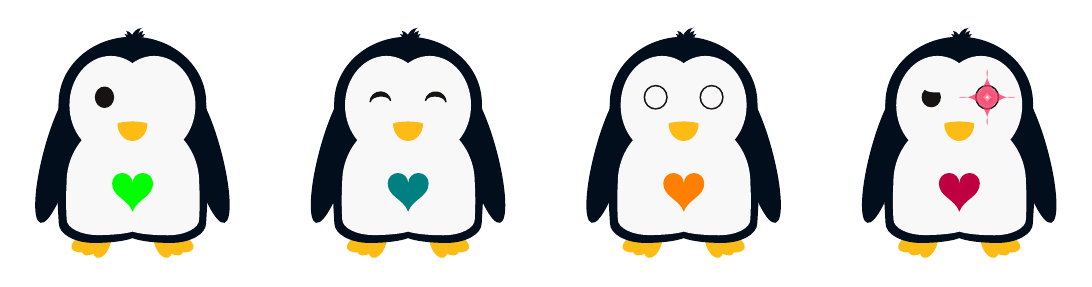
\begin{tikzpicture}
	\pingu[left eye none, heart=green]
	\pingu[eyes wink, heart=teal, xshift=3.5cm]
	\pingu[eyes shock,  heart=orange, xshift=7cm]
	\pingu[left eye devil, right eye angry, heart=purple,  xshift=10.5cm]
\end{tikzpicture}
\end{tcblisting}

\subsection{Changing other components}
Just like for the wings and the eyes, you can change th following body parts:
\begin{itemize}
	\item The \textit{feet} (again with separate left and right)\\*
		Select from: \typesetselection{leftfoot}.
	\item The \textit{bill} (does not have left and right, as there is just one)\\*
		Select from: \typesetselection{bill}.
	\item The \textit{hairstyle} (does not have left and right)\\*
		Select from: \typesetselection{hairstyle}.
\end{itemize}
For each selection, \say{none} will prohibit the drawing, and \say{normal} is the default chosen.
\begin{tcblisting}{sidebyside=false, title=Bodyparts-Showcase}
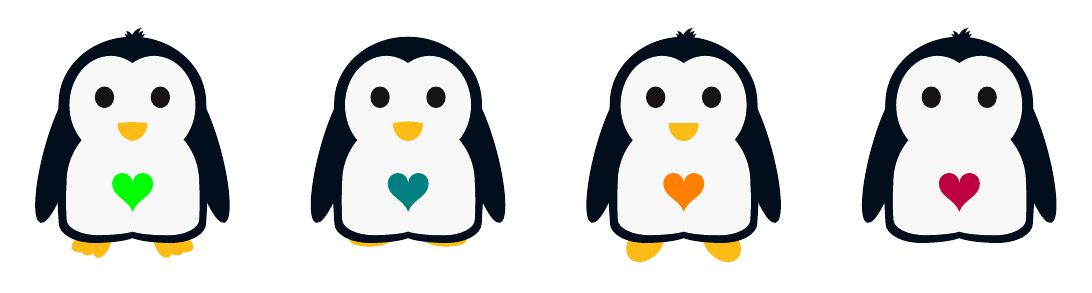
\begin{tikzpicture}
	\pingu[bill angry, heart=green]
	\pingu[feet back, hairstyle none, heart=teal, xshift=3.5cm]
	\pingu[bill flat, feet simple, heart=orange, xshift=7cm]
	\pingu[feet none, bill none, heart=purple, xshift=10.5cm]
\end{tikzpicture}
\end{tcblisting}

\subsection{Predefined Styles}
While the penguin options offer the modification of basically every drawing routine (through other styles like |@block|), it is tedious to change them every time.
So I have started to create some predefined styles, that do change some of the penguins appearance (and are completely new, so beware of bugs):
\begin{multicols}{2}
\begin{itemize}
	\foreach \tx/\s in {{draw everything with a line}/{:line}, {draw components with transparency}/{:ghost parts}, {draw all layers with transparency}/{:ghost}, {set all of the \say{devil}-components}/{:devil},{flip the penguin (swaps left \& right)}/{:back}} {
		\item \parbox[t]{.8\linewidth}{\raggedright\texttt{\s}, \tx.} \hfill
		\parbox[t]{.175\linewidth}{\scalebox{.4}{%
			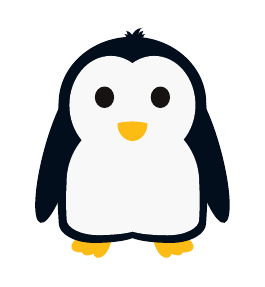
\begin{tikzpicture}[baseline=.35\baselineskip]%
				\pingu[\s]
			\end{tikzpicture}%
		}}
	}
	\item[] \parbox[t][2.4\baselineskip]{0pt}{}% buffer
\end{itemize}
\end{multicols}
Currently, only some of the styles do affect other items. As an example, consider |:line|, that changes the draw-style of wing-items and extras:
\begin{tcblisting}{title={Line Penguin}}
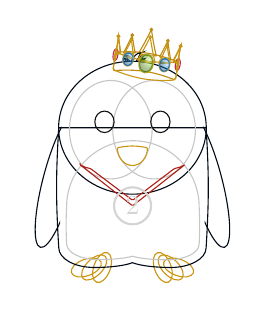
\begin{tikzpicture}
	\pingu[:line, princess crown, silver medal]
\end{tikzpicture}
\end{tcblisting}

\subsection{Extras}
An extra is considered everything, that is attached to the main penguin and not to the wings (as those items may be placed separately for both wings).
Most extras are activated with the format |<extra>=<color>| (the |<color>| option is not mandatory)
and try to adapt with other extras that have been placed (yet you can place multiple hats if you really like to).  A lot of the extras do offer more keys to customize their appearance.
They are explained in the full reference (\autoref{sec:full-ref}).

Consider the following, somewhat overkill-example:
\begin{tcblisting}{title={Lord-Gadget, the penguin}}

\begin{tikzpicture}
	\pingu[crown 2d=pingu@bronze,
	       medal=pingu@purple, tie,
	       eye patch left=teal,
	       eye patch right=orange,
	       right wing wave, sunglasses,
	       glow thick=yellow]
\end{tikzpicture}
\end{tcblisting}

\subsection{Wing-Items}

\section{Examples}

\appendix
\section{Full Reference}\label{sec:full-ref}

\end{document}